\documentclass[]{scrartcl}
\usepackage{graphicx}
\usepackage{hyperref}

%opening
\title{Network interpretability}
\author{Guillermo Romero Moreno}

\begin{document}

\maketitle

\tableofcontents

\newpage
I used Keras \cite{chollet2015keras}
I did not

\section{Introduction: neural networks interpretability}
"There is a growing sense that neural networks need to be interpretable to humans. The field of neural network interpretability has formed in response to these concerns. As it matures, two major threads of research have begun to coalesce: feature visualization and attribution. 

\textbf{Feature visualization} answers questions about what a network — or parts of a network — are looking for by generating examples.

\textbf{Attribution} (or saliency maps) studies what part of an example is responsible for the network activating a particular way." \cite{Olah2017}

"One of the challenges of neural networks is understanding what exactly goes on at each layer.
We know that after training, each layer progressively extracts higher and higher-level features of the image, until the final layer essentially makes a decision on what the image shows.
For example, the first layer maybe looks for edges or corners.
Intermediate layers interpret the basic features to look for overall shapes or components, like a door or a leaf.
The final few layers assemble those into complete interpretations---these neurons activate in response to very complex things such as entire buildings or trees." \cite{Mordvintsev2015}

"Deep neural networks are highly expressive models that have recently achieved state of the art performance on speech and visual recognition tasks. While their expressiveness is the reason they succeed, it also causes them to learn uninterpretable solutions that could have counter-intuitive properties." \cite{Szegedy2013}

"Nonlinear methods such as Deep Neural Networks (DNNs) are the gold standard for various challenging machine learning problems, e.g., image classification, natural language processing or human action recognition. Although these methods perform impressively well, they have a significant disadvantage, the lack of transparency, limiting the interpretability of the solution and thus the scope of application in practice. Especially DNNs act as black boxes due to their multilayer nonlinear structure.
[...]
An interpretable classifier explains its nonlinear classification decision in terms of the inputs. For instance, in image classification problems, the classifier should not only indicate whether an image of interest belongs to a certain category or not, but also explain what structures (e.g. pixels in the image) were the basis for its decision (cf. Figure 1). This additional information helps to better assess the quality of a particular prediction, or to verify the overall reasoning ability of the trained classifier. Also, information about which pixels are relevant in a particular image, could be used for determining which region of the image should be the object of further anal- ysis. Linear models readily provide explanations in terms of input variables (see for example [19], [20]). However, because of the limited expressive power of these models, they perform poorly on complex tasks such as image recognition. Extending linear analysis techniques to more realistic nonlinear models such as deep neural networks, is therefore of high practicala relevance." \cite{Montavon2017}
\begin{figure}
\centering
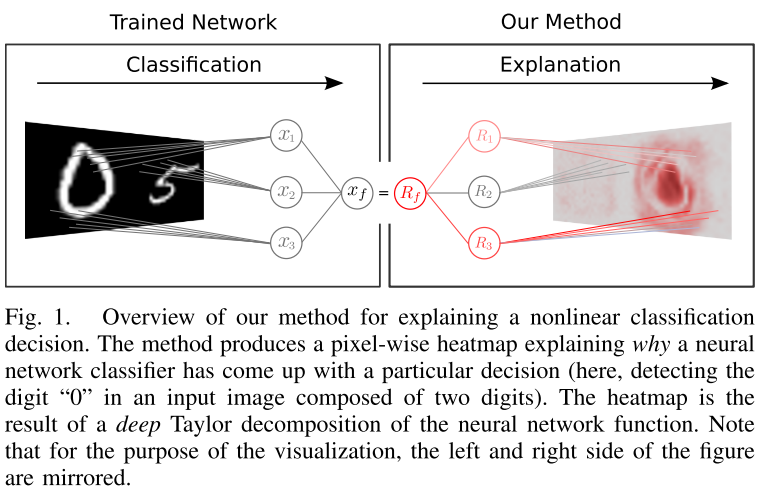
\includegraphics[width=0.7\linewidth]{deeptaylor}\\
\end{figure}

"Networks with Rectified Linear Units (ReLUs) create nonlinearities that must be addressed. Several variants exist for handling this [448,454]. Backpropagation-based methods are a highly active area of research. Researchers are still actively identifying weaknesses [455], and new methods are being developed to address them [219,456,457]. Lundberg and Lee [458] noted that several importance scoring methods including integrated gradients and LIME could all be considered approximations to Shapely values [459], which have a long history in game theory for assigning contributions to players in cooperative games." \cite{Ching2017}

"The purported “black box” nature of neural networks is a barrier to adoption in applica- tions where interpretability is essential." \cite{Shrikumar2017}

\subsection{In biological sequences}
"In recent years, there has been an explosion of deep learning models which have lead to groundbreaking results in many fields such as computer vision[13], natural language processing[25], and computational biology [2, 19, 27, 11, 14, 22]. However, although these models have proven to be very accurate, they have widely been viewed as “black boxes” due to their complexity, making them hard to understand. This is particularly unfavorable in the biomedical domain, where understanding a model’s predictions is extremely important for doctors and researchers trying to use the model.
[...]
While making accurate predictions is important in biomedical tasks, it is equally important to understand why models make their predictions. Accurate, but uninterpretable models are often very slow to emerge in practice due to the inability to understand their predictions, making biomedical domain experts reluctant to use them. Consequently, we aim to obtain a better understanding of why certain models work better than others, and investigate how they make their predictions by introducing several visualization techniques.
[...]
The main difference between our work and previous works on images and natural language is that instead of trying to understand the DNNs given human understanding of such human perception tasks, we attempt to uncover critical signals in DNA sequences given our understanding of DNNs." \cite{Lanchantin2016}

\section{Feature visualization}

"While quantitative analyses and comparisons of such models exist, and visualizations of the first layer representations are common in the literature, one area where more work needs to be done is the qualitative analysis of representations learned beyond the first level. [...] Our aim was to explore ways of visualizing what a unit computes in an arbitrary layer of a deep network. The goal was to have this visualization in the input space (of images), to have an efficient way of computing it, and to make it as general as possible (in the sense of it being applicable to a large class of neural-network-like models)." \cite{Erhan2009}

\subsection{Linear combination of filters}
"Lee et al. (2008) showed one way of visualizing what the units in the second hidden layer of a network are responding to. They made the assumption that a unit can be characterized by the filters of the previous layer to which it is most strongly connected (i.e. whose weight to the upper unit is large in magnitude). By taking a weighted linear combination of the previous layer filters [...].
Lee et al. (2009) used an extended version of this method for visualizing units of the third layer [...].
Such a technique is simple and efficient. One disadvantage is that it is not clear how to automatically choose the appropriate number of filters to keep at each layer. [...], this method also bypasses the nonlinearities between layers" \cite{Erhan2009}
\subsubsection{In biological sequences}
"The networks whose filters were saved and plotted only used one-hot encoding so as to be able to represent all features as PSSM-logos. The visualization of the convolutional filters was based on the methodology used in [37]. The convolutional filters are represented as a matrix of filter\_width columns and aa\_encoding rows. So as to visualize the relative importance of each of the positions in the filter, each of them is rescaled in a way that the height of the highest column is 1. After this transformation, each filter can be visualized as a PSSM logo where the position importance is proportional to the height of the column and the height of each letter is proportional to the importance of the amino acid in that position. Seq2logo [42] is used in order to generate the PSSM-logo plots. The Seq2Logo default amino acid colour coding is used: negatively charged (DE) residues are red, polar uncharged residues (NQSGTY) are green, positively charged (RKH) residues are blue and the remaining are black." \cite{Fontal2017}

"For TFBS prediction, Alipanahi et al.[2] was the first to implement a visualization method on a DNN model. They visualize their CNN model by extracting motifs based on the input subsequence corresponding to the strongest activation location for each convolutional filter (which we call convolution activation). Since they only have one convolutional layer, it is trivial to map the activations back, but this method does not work as well with deeper models. We attempted this technique on our models and found that our approach using saliency maps outperforms it in finding motif patterns (details in section 4). Quang and Xie [19] use the same visualization method on their convolutional-recurrent model for noncoding variant prediction." \cite{Lanchantin2016}

\subsection{Activation maximization}
"we look for input patterns of bounded norm which maximize the activation of a given hidden unit (The total sum of the input to the unit from the previous layer plus its bias.); since the activation function of a unit in the first layer is a linear function of the input, in the case of the first layer, this input pattern is proportional to the filter itself. [...] 
One simple way of doing this is to find, for a given unit, the input sample(s) (from either the training or the test set) that give rise to the highest activation of the unit. Unfortunately, this still leaves us with the problem of choosing how many samples to keep for each unit and the problem of how to “combine” these samples. Ideally, we would like to find out what these samples have in common. Furthermore, it may be that only some subsets of the input vector contribute to the high activation, and it is not easy to determine which by inspection.
[...]
maximizing the activation of a unit as an optimization problem.
\begin{equation}
x* = arg \max\limits_{x \; s.t. ||x||=\rho} h_{ij}(\theta,x)
\end{equation}
This is, in general, a non-convex optimization problem. But it is a problem for which we can at least try to find a local minimum. This can be done most easily by performing simple gradient ascent in the input space [...] 
the unit can then be characterized by the minimum or set of minima found. In the latter case, one can either average the results, or choose the one which maximizes the activation, or display all the local minima obtained to characterize that unit.
This optimization technique (we will call it “activation maximization”) does involve a choice of hyperparameters: the learning rate and a stopping criterion" \cite{Erhan2009}

"the response of an internal unit to input images, as a function in image space, appears to be unimodal, or at least that the maximum is found reliably and consistently for all the random initializations tested. This is interesting because finding this dominant mode is relatively easy, and displaying it then provides a good characterization of what the unit does." \cite{Erhan2009}

"We tested the activation maximization procedure on image patches of 20 × 20 pixels (instead of 12×12) and found that the optimization does not converge to a single global minimum. Moreover, the input distribution that is sampled with the units clamped to 1 has many different modes and its expectation is not meaningful or interpretable any-more. [...] 
It is perhaps unrealistic to expect that as we scale the datasets to larger and larger images, one could still find a simple representation of a higher layer unit. We should note, however, that there is a recent trend of developing convolutional versions of deep architectures (Kavukcuoglu et al., 2009; Lee et al., 2009; Desjardins \& Bengio, 2008): it is likely that one will be able to apply the same techniques in that scenario and still be able to recover good visualizations, even with large inputs." \cite{Erhan2009}

"One way to visualize what goes on is to turn the network upside down and ask it to enhance an input image in such a way as to elicit a particular interpretation. Say you want to know what sort of image would result in “Banana.” Start with an image full of random noise, then gradually tweak the image towards what the neural net considers a banana (see related work in [1], [2], [3], [4]). By itself, that doesn’t work very well, but it does if we impose a prior constraint that the image should have similar statistics to natural images, such as neighboring pixels needing to be correlated." \cite{Mordvintsev2015}

"Neural networks are, generally speaking, differentiable with respect to their inputs. If we want to find out what kind of input would cause a certain behavior --- whether that's an internal neuron firing or the final output behavior --- we can use derivatives to iteratively tweak the input towards that goal [3]." \cite{Olah2017}
\begin{figure}[h]
	\centering
	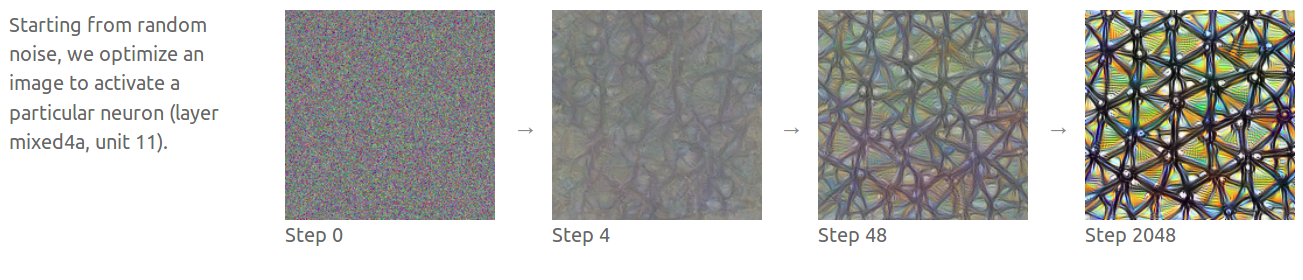
\includegraphics[width=1\linewidth]{randopt}
\end{figure}

" Optimization can give us an example input that causes the desired behavior --- but why bother with that? Couldn't we just look through the dataset for examples that cause the desired behavior?

It turns out that optimization approach can be a powerful way to understand what a model is really looking for, because it separates the things causing behavior from things that merely correlate with the causes. [...] A neuron may not be detecting what you initially thought. Optimization also has the advantage of flexibility. For example, if we want to study how neurons jointly represent information, we can easily ask how a particular example would need to be different for an additional neuron to activate. This flexibility can also be helpful in visualizing how features evolve as the network trains. If we were limited to understanding the model on the fixed examples in our dataset, topics like these ones would be much harder to explore. " \cite{Olah2017}
\begin{figure}[h]
	\centering
	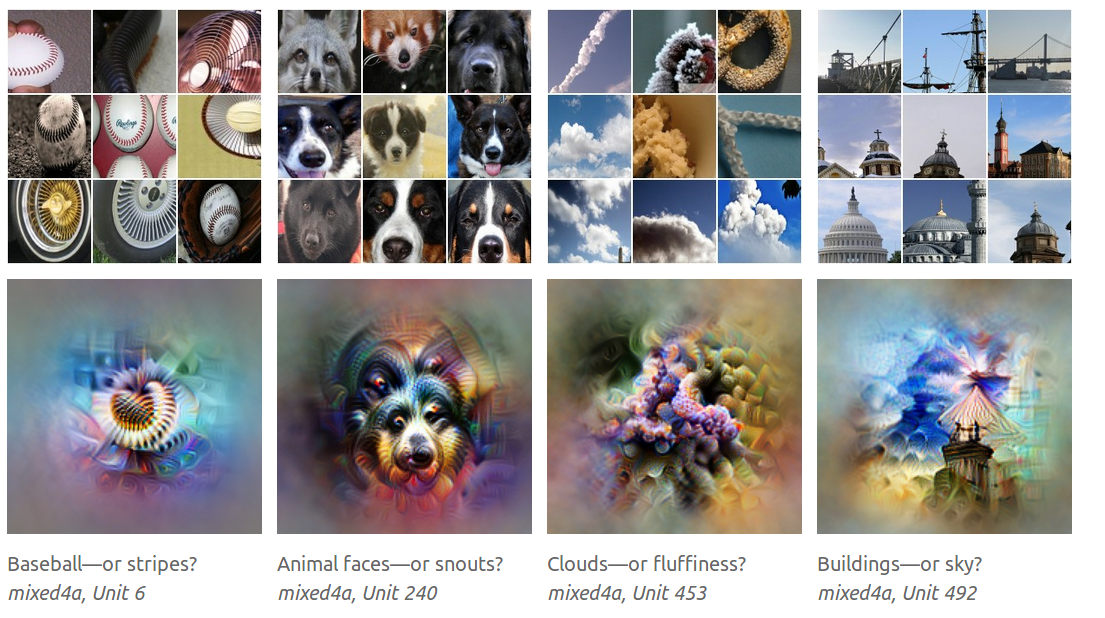
\includegraphics[width=1\linewidth]{optimization}
\end{figure}

\subsubsection{Units vs channels vs layers}
"If we want to understand individual features, we can search for examples where they have high values --- either for a neuron at an individual position, or for an entire channel. We used the channel objective to create most of the images in this article." \cite{Olah2017}
\begin{figure}[h]
	\centering
	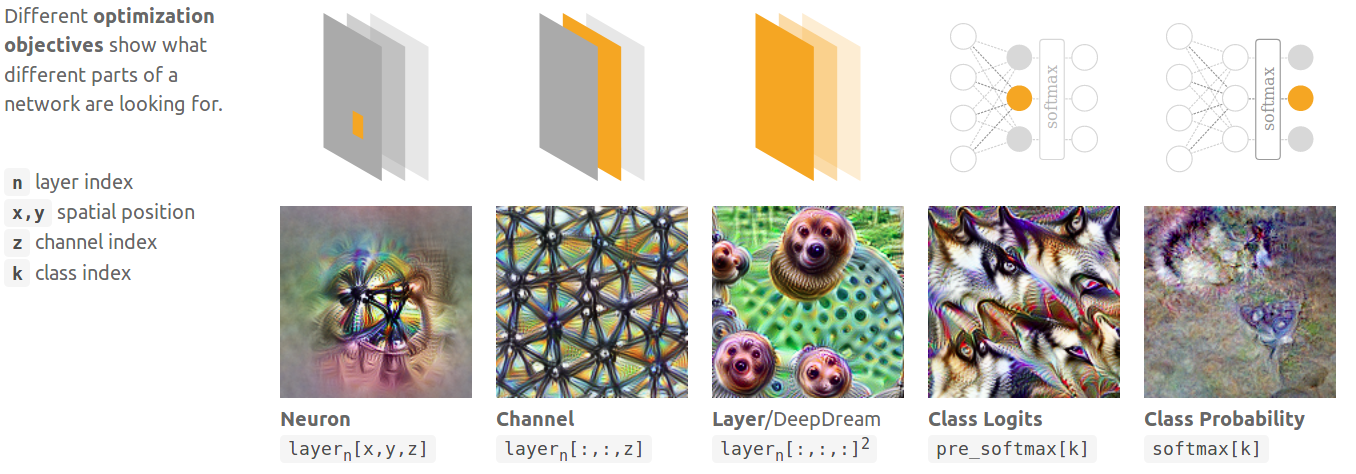
\includegraphics[width=1\linewidth]{diffopt}
\end{figure}

"First, we find that there is no distinction between individual high level units and random linear combinations of high level units, according to various methods of unit analysis. It suggests that it is the space, rather than the individual units, that contains the semantic information in the high layers of neural networks.
[...]
The inspection of individual units makes the implicit assumption that the units of the last feature layer form a distinguished basis which is particularly useful for extracting semantic information. Instead, we show in section 3 that random projections of φ(x) are semantically indistinguishable from the coordinates of φ(x). This puts into question the conjecture that neural networks disentangle variation factors across coordinates. Generally, it seems that it is the entire space of activations, rather than the individual units, that contains the bulk of the semantic information." \cite{Szegedy2013}

"Second, we find that deep neural networks learn input-output mappings that are fairly discontinuous to a significant extent. We can cause the network to misclassify an image by applying a certain hardly perceptible perturbation, which is found by maximizing the network’s prediction error. [...] We term the so perturbed examples “adversarial examples”. [...] we found that adversarial examples are relatively robust, and are shared by neural networks with varied number of layers, activations or trained on different subsets of the training data.
[...]
In addition, the specific nature of these perturbations is not a random artifact of learning: the same perturbation can cause a different network, that was trained on a different subset of the dataset, to misclassify the same input." \cite{Szegedy2013}

"Traditional computer vision systems rely on feature extraction: often a single feature is easily inter- pretable, e.g. a histogram of colors, or quantized local derivatives. This allows one to inspect the individual coordinates of the feature space, and link them back to meaningful variations in the input domain. Similar reasoning was used in previous work that attempted to analyze neural networks that were applied to computer vision problems. These works interpret an activation of a hidden unit as a meaningful feature. They look for input images which maximize the activation value of this single feature [6, 7] \cite{Zeiler2014} \cite{Erhan2009}. [...] So far, unit-level inspection methods had relatively little utility beyond confirming certain intuitions regarding the complexity of the representations learned by a deep neural network." \cite{Szegedy2013}

"Diversity also starts to brush on a more fundamental issue: while the examples above represent a mostly coherent idea, there are also neurons that represent strange mixtures of ideas. Below, a neuron to responds to two types of animal faces, and also to car bodies. Examples like these suggest that neurons are not necessarily the right semantic units for understanding neural nets.  In real life, combinations of neurons work together to represent images in neural networks. Individual neurons are the basis directions of activation space, and it is not clear that these should be any more special than any other direction. \cite{Szegedy2013} found that random directions seem just as meaningful as the basis directions. More recently Bau, Zhou et al.[12] found basis directions to be interpretable more often than random directions. Our experience is broadly consistent with both results; we find that random directions often seem interpretable, but at a lower rate than basis directions. We can also define interesting directions in activation space by doing arithmetic on neurons. For example, if we add a “black and white” neuron to a “mosaic” neuron, we obtain a black and white version of the mosaic. This is reminiscent of semantic arithmetic of word embeddings as seen in Word2Vec or generative models’ latent spaces. These examples show us how neurons jointly represent images. To better understand how neurons interact, we can also interpolate between them. This is similar to interpolating in the latent space of generative models. The optimization objective is a linear interpolation between the individual channel objectives. To get the interpolations to look better, we also add a small alignment objective that encourages lower layer activations to be similar. We additionally use a combination of separate and shared image parameterizations to make it easier for the optimization algorithm to cause objects to line up, while still giving it the freedom to create any image it needs to. This is only starting to scratch the surface of how neurons interact. The truth is that we have almost no clue how to select meaningful directions, or whether there even exist particularly meaningful directions. Independent of finding directions, there are also questions on how directions interact — for example, interpolation can show us how a small number of directions interact, but in reality there are hundreds of directions interacting.

If you want to visualize features, you might just optimize an image to make neurons fire. Unfortunately, this doesn’t really work. Instead, you end up with a kind of neural network optical illusion — an image full of noise and nonsensical high-frequency patterns that the network responds strongly to. These patterns seem to be the images kind of cheating, finding ways to activate neurons that don’t occur in real life. If you optimize long enough, you’ll tend to see some of what the neuron genuinely detects as well, but the image is dominated by these high frequency patterns. These patterns seem to be closely related to the phenomenon of adversarial examples [11]. We don’t fully understand why these high frequency patterns form, but an important part seems to be strided convolutions and pooling operations, which create high-frequency patterns in the gradient [13]. These high-frequency patterns show us that, while optimization based visualization’s freedom from constraints is appealing, it’s a double-edged sword. Without any constraints on images, we end up with adversarial examples. These are certainly interesting, but if we want to understand how these models work in real life, we need to somehow move past them..." \cite{Olah2017}

"If we want to understand a layer as a whole, we can use the DeepDream objective [4], searching for images the layer finds 'interesting.'" \cite{Olah2017}
\subsubsection{Outputs}
"And if we want to create examples of output classes from a classifier, we have two options --- optimizing class logits before the softmax or optimizing class probabilities after the softmax. One can see the logits as the evidence for each class, and the probabilities as the likelihood of each class given the evidence. \textbf{Unfortunately, the easiest way to increase the probability softmax gives to a class is often to make the alternatives unlikely rather than to make the class of interest likely} \cite{Simonyan2014}. From our experience, optimizing pre-softmax logits produces images of better visual quality. an alternate hypothesis is that it’s just harder to optimize through the softmax function. We understand this has sometimes been an issue in adversarial examples, and the solution is to optimize the LogSumExp of the logits instead. This is equivalent to optimizing softmax but generally more tractable. Our experience was that the LogSumExp trick doesn’t seem better than dealing with the raw probabilities. Regardless of why that happens, it can be fixed by very strong regularization with generative models. In this case the probabilities can be a very principled thing to optimize." \cite{Olah2017}
\subsubsection{Diversity}
"Do our examples show us the full picture? When we create examples by optimization, this is something we need to be very careful of. It’s entirely possible for genuine examples to still mislead us by only showing us one “facet” of what a feature represents.  Dataset examples have a big advantage here. By looking through our dataset, we can find diverse examples. It doesn't just give us ones activating a neuron intensely: we can look across a whole spectrum of activations to see what activates the neuron to different extents. In contrast, optimization generally gives us just one extremely positive example --- and if we’re creative, a very negative example as well." \cite{Olah2017}
\begin{figure}[h]
	\centering
	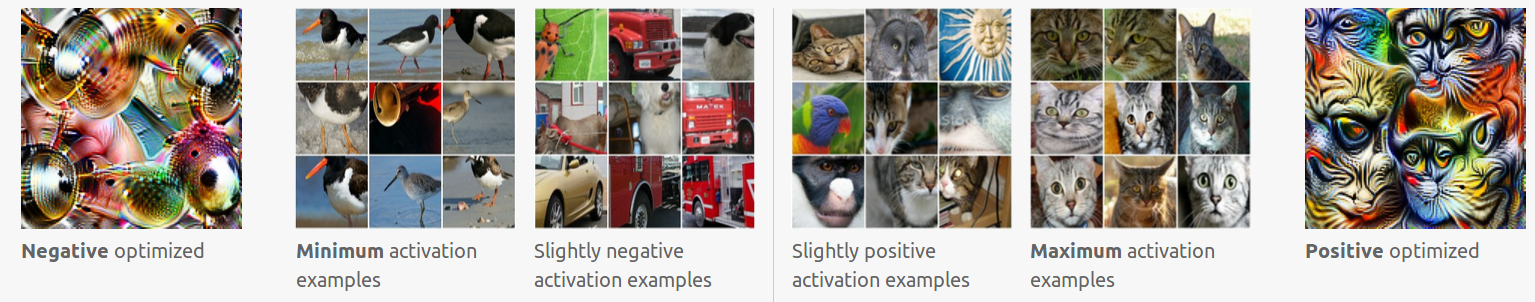
\includegraphics[width=1\linewidth]{Diversity}
\end{figure}
"A given feature of a network may respond to a wide range of inputs. On the class level, for example, a classifier that has been trained to recognize dogs should recognize both closeups of their faces as well as wider profile images --- even though those have quite different visual appearances. Early work by Wei et al.[8] attempts to demonstrate this “intra-class” diversity by recording activations over the entire training set, clustering them and optimizing for the cluster centroids, revealing the different facets of a class that were learned. A different approach by Nguyen, Yosinski, and collaborators was to search through the dataset for diverse examples and use those as starting points for the optimization process [9]. The idea is that this initiates optimization in different facets of the feature so that the resulting example from optimization will demonstrate that facet. In more recent work, they combine visualizing classes with a generative model, which they can sample for diverse examples [10]. Their first approach had limited success, and while the generative model approach works very well --- we’ll discuss it more in the section on regularization under learned priors --- it can be a bit tricky. " \cite{Olah2017}
\begin{figure}[h]
	\centering
	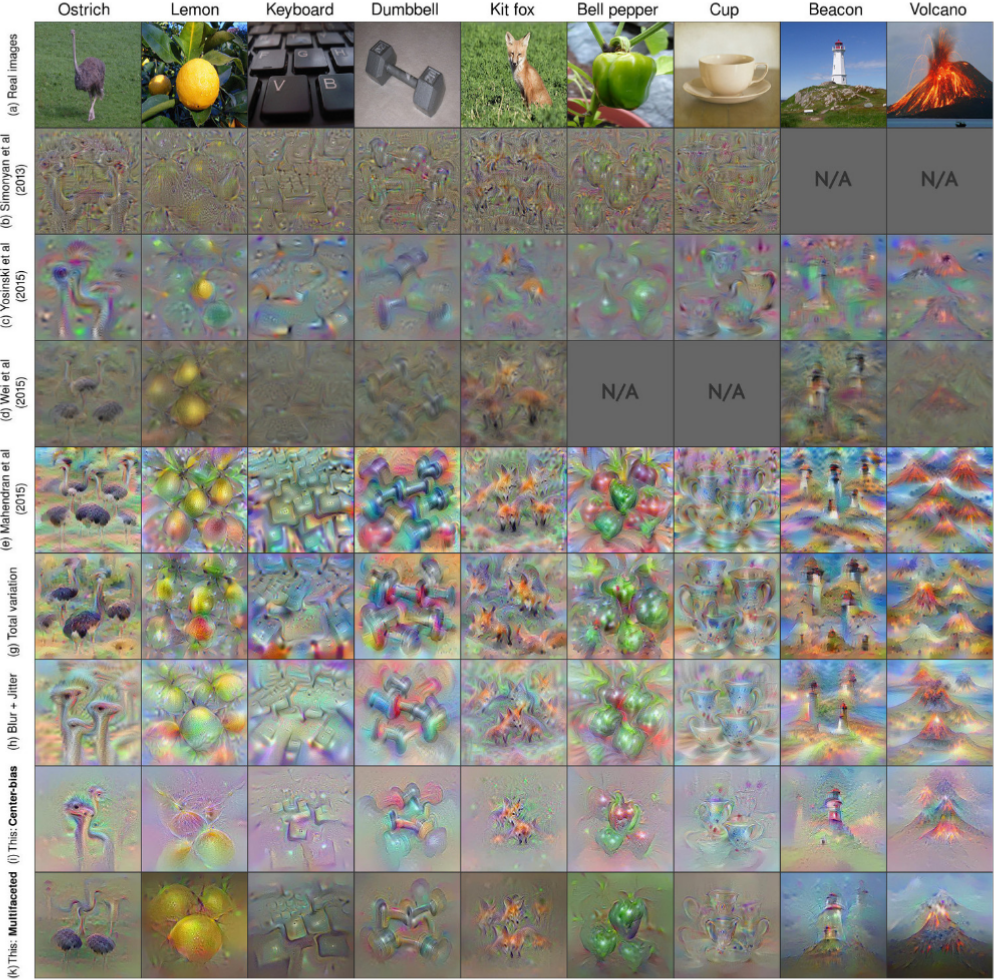
\includegraphics[width=1\linewidth]{multifaceted}
\end{figure}
"We find there’s a very simple way to achieve diversity: adding a “diversity term” to one’s objective that pushes multiple examples to be different from each other. The diversity term can take a variety of forms, and we don’t have much understanding of their benefits yet. One possibility is to penalize the cosine similarity of different examples. Another is to use ideas from style transfer [6] to force the feature to be displayed in different styles. For this article we use an approach based on ideas from artistic style transfer. Following that work, we begin by computing the Gram matrix GGG of the channels, where: $G_{i,j} = layer_n[:, :, i] \cdot layer_n[:, :, j]$. From this, we compute the diversity term: the negative pairwise cosine similarity of pairs of visualizations. $C_{diversity} = - \sum_{a} \sum_{b\neq a} ~ \frac{vec(G_a) \cdot vec(G_b)}{||vec(G_a)||~||vec(G_b)||}$.​ We then maximize the diversity term jointly with the regular optimization objective. In lower level neurons, a diversity term can reveal the different facets a feature represents. [...] The effect of diversity can be even more striking in higher level neurons, where it can show us different types of objects that stimulate a neuron. This simpler approach has a number of shortcomings: For one, the pressure to make examples different can cause unrelated artifacts (such as eyes) to appear. Additionally, the optimization may make examples be different in an unnatural way. For example, in the above example one might want to see examples of soccer balls clearly separated from other types of balls like golf or tennis balls. Dataset based approaches such as Wei et al.[8] can split features apart more naturally — however they may not be as helpful in understanding how the model will behave on different data. " \cite{Olah2017}
\subsubsection{Regularization}
"We can think of all of these approaches as living on a spectrum, based on how strongly they regularize the model. On one extreme, if we don’t regularize at all, we end up with adversarial examples. On the opposite end, we search over examples in our dataset and run into all the limitations we discussed earlier. And in the middle we have three main families of regularization options." \cite{Olah2017}
\begin{figure}[h]
	\centering
	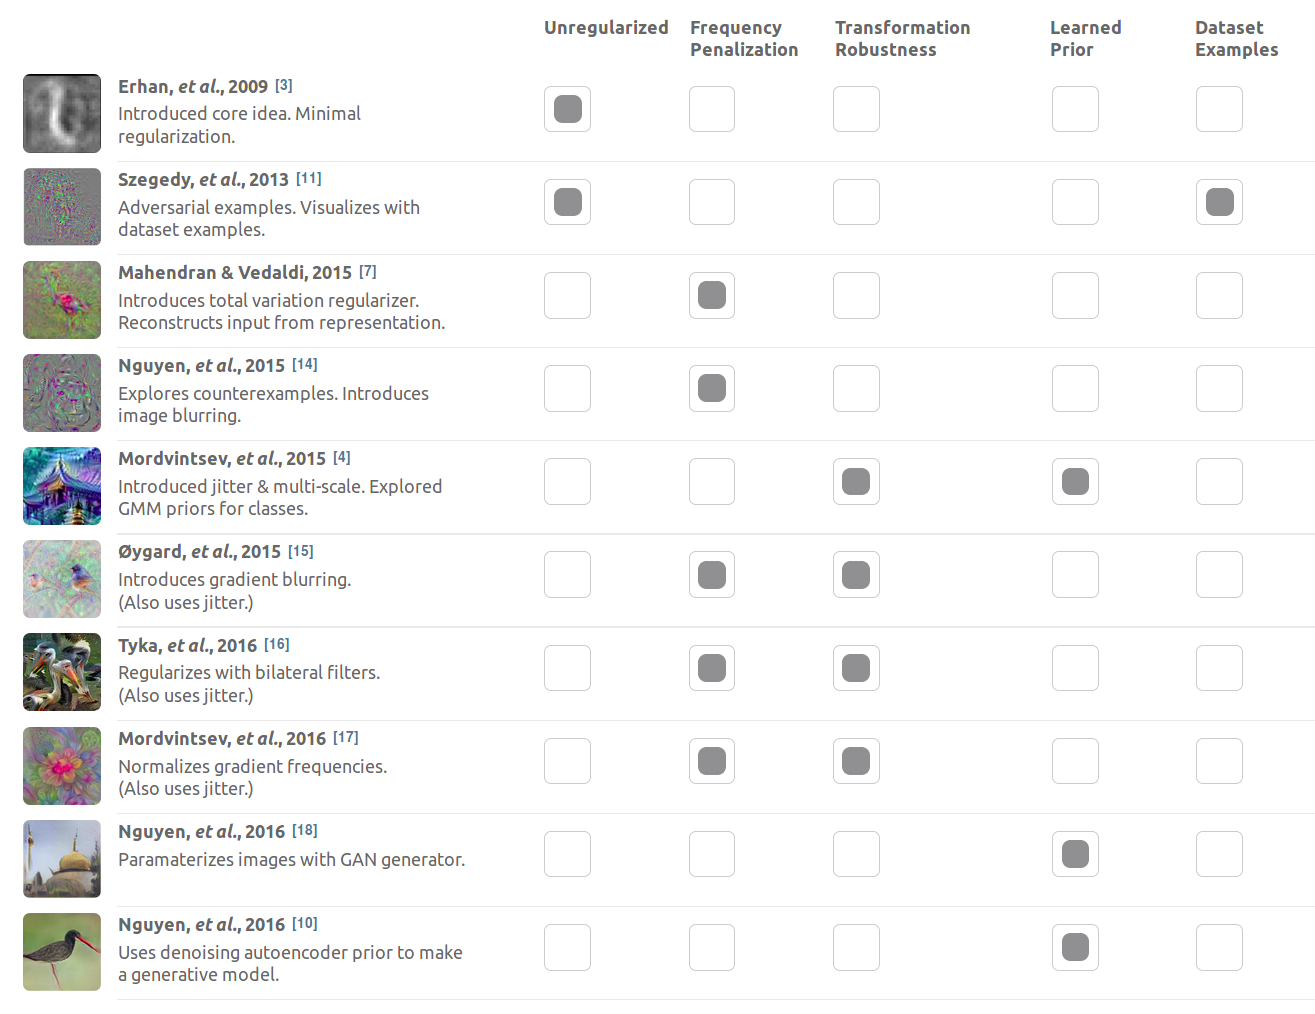
\includegraphics[width=1\linewidth]{regularization}
\end{figure}
"Let’s consider these three intermediate categories of regularization in more depth.

\textbf{Frequency penalization} directly targets the high frequency noise these methods suffer from. It may explicitly penalize variance between neighboring pixels (total variation) [7], or implicitly penalize high-frequency noise by blurring the image each optimization step [14]. If we think about blurring in Fourier space, it is equivalent to adding a scaled L2 penalty to the objective, penalizing each Fourier-component based on its frequency. Unfortunately, these approaches also discourage legitimate high-frequency features like edges along with noise. This can be slightly improved by using a bilateral filter, which preserves edges, instead of blurring [16].
(Some work uses similar techniques to reduce high frequencies in the gradient before they accumulate in the visualization [15, 17]. These techniques are in some ways very similar to the above and in some ways radically different --- we’ll examine them in the next section, Preconditioning and Parameterization.)

\textbf{Transformation robustness} tries to find examples that still activate the optimization target highly even if we slightly transform them. Even a small amount seems to be very effective in the case of images [4], especially when combined with a more general regularizer for high-frequencies [15, 17]. Concretely, this means that we stochastically jitter, rotate or scale the image before applying the optimization step.

\textbf{Learned priors.} Our previous regularizers use very simple heuristics to keep examples reasonable. A natural next step is to actually learn a model of the real data and try to enforce that. With a strong model, this becomes similar to searching over the dataset. This approach produces the most photorealistic visualizations, but it may be unclear what came from the model being visualized and what came from the prior.
One approach is to learn a generator that maps points in a latent space to examples of your data, such as a GAN or VAE, and optimize within that latent space [18]
. An alternative approach is to learn a prior that gives you access to the gradient of probability; this allows you to jointly optimize for the prior along with your objective [10, 4]. When one optimizes for the prior and the probability of a class, one recovers a generative model of the data conditioned on that particular class. Finally, Wei et al.[8] approximate a generative model prior, at least for the color distribution, by penalizing distance between patches of the output and the nearest patches retrieved from a database of image patches collected from the training data." \cite{Olah2017}
	\subsubsection{Preconditioning}
	"In the previous section, we saw a few methods [15, 17] that reduced high frequencies in the gradient rather than the visualization itself. It’s not clear this is really a regularizer: it resists high frequencies, but still allows them to form when the gradient consistently pushes for it. If it isn’t a regularizer, what does transforming the gradient like this do? Transforming the gradient like this is actually quite a powerful tool --- it’s called “preconditioning” in optimization. You can think of it as doing steepest descent to optimize the same objective, but in another parameterization of the space or under a different notion of distance. 6 This changes which direction of descent will be steepest, and how fast the optimization moves in each direction, but it does not change what the minimums are. If there are many local minima, it can stretch and shrink their basins of attraction, changing which ones the optimization process falls into. As a result, using the right preconditioner can make an optimization problem radically easier. Gradient blurring [15] is equivalent to gradient descent in a different parameterization of image space, where high frequency dimensions are stretched to make moving in those directions slower. Gradient Laplacian Pyramid normalization [17] is a kind of adaptive learning rate approach in the same space.
	How can we choose a preconditioner that will give us these benefits? A good first guess is one that makes your data decorrelated and whitened. In the case of images this means doing gradient descent in the Fourier basis, 7 with frequencies scaled so that they all have equal energy. Note that we have to be careful to get the colors to be decorrelated, too. The Fourier transforms decorrelates spatially, but a correlation will still exist between colors. To address this, we explicitly measure the correlation between colors in the training set and use a Cholesky decomposition to decorrelate them. Let’s see how using different measures of distance changes the direction of steepest descent. The regular L2 gradient can be quite different from the directions of steepest descent in the L∞ metric or in the decorrelated space [...]. Notice that optimizing in the decorrelated space reduces high frequencies, while using L∞ increases them. Using the decorrelated descent direction results in quite different visualizations. It’s hard to do really fair comparisons because of hyperparameters, but the resulting visualizations seem a lot better --- and develop faster, too.
	Is the preconditioner merely accelerating descent, bringing us to the same place normal gradient descent would have brought us if we were patient enough? Or is it also regularizing, changing which local minima we get attracted to? It’s hard to tell for sure. On the one hand, gradient descent seems to continue improving as you exponentially increase the number of optimization steps — it hasn't converged, it's just moving very slowly. On the other hand, if you turn off all other regularizers, the preconditioner seems to reduce high-frequency patterns." \cite{Olah2017}
	
	"In order to focus on higher probable regions of the input space, the
	2-norm regularizer can be replaced by a data density model p(x) which is called “expert” by Montavon et al.(2017). This leads to the following optimization problem:
	max x log p(ωc|x) + log p(x).
	Here, the prototype is encouraged to simultaneously produce strong class response and to  resemble  the  data.   By  application  of  Bayes’  rule,  the  newly  defined  objective  can  be identified, up to modeling errors and a constant term, as the class-conditioned data density p(x|ωc).  The learned prototype thus corresponds to the most likely input x for the class ωc.  A possible choice for the expert is the Gaussian Restricted Boltzmann Machine (RBM).
	The RBM is a two-layer, bipartite, undirected graphical model with a set of binary hidden units p(h), a set of (binary or real-valued) visible units p(v), with symmetric connections between the two layers represented by a weight matrix W.  The probabilistic semantics for an RBM is defined by its energy function" \cite{Montavon2018}
	
	\subsubsection{In proteins}
	"In the case of the NN trained in this project, where the inputs are protein sequences encoded as one-hot vectors, the optimized inputs lose the one-hot vector encoding but can be forced to behave as a Position Probability Matrix (PPM) which can then be represented as a motif. Formally, the following equation, where Si is the score (defined as the unscaled values for class Ci pre Softmax transformation) and X is the input sequence, is optimized:
	arg max Si(X) + λ ? X ?2 2.
	λ is the regularisation parameter. The L2-regularization term is introduced in order to minimize the number of significant amino acids per position in the optimized input sequence. The score used is the value of the pre-Softmax layer because the post-Softmax value can be maximized by just minimizing the scores of the other classes, and the objective is to get an ideal input for the desired class, not an input modified to score low in the remaining classes." \cite{Fontal2017}
	
	"Now we introduce an approach to extract a class-specific visualization for a DNN model, where we attempt to find the best sequence which maximizes the probability of a positive TFBS, which we call class optimization. Formally, we optimize the following equation where S+(X) is the probability (or score) of an input sequence X (matrix in our case) being a positive TFBS computed by the softmax equation of our trained DNN model for a specific TF:
	arg maxS+(X) + λ?X?2 2
	where λ is the regularization parameter. We find a locally optimal X through stochastic gradient descent, where the optimization is with respect to the input sequence. In this optimization, the model weights remain unchanged. This is similar to the methods used in Simonyan et al.[21] to optimize toward a specific image class. This visualization method depicts the notion of a positive TFBS class for a particular TF and is not specific to any test sequence." \cite{Lanchantin2016}
	
	"The optimization is done via Adam [15] changing only the values of the input sequence. Initial values are all set as 1/20 to give equal probability to each amino acid in each position. λ = 0.00005. At the end of each optimization step, the values are forced to stay withing a realistic range:
	• Negative values are converted to 0.
	• The values for each position are standardized in order to make the total sum equal to 1.
	After a certain number of optimization steps, the final sequence is recovered and represented as a motif logo using Seq2Logo [42]." \cite{Fontal2017}

	\subsubsection{Others}
	The objectives we've mentioned only scratch the surface of possible objectives --- there are a lot more that one could try. Of particular note are the objectives used in style transfer \cite{Gatys2016}, which can teach us about the kinds of style and content a network understands, and objectives used in optimization-based model inversion \cite{Mahendran2015}, which help us understand what information a model keeps and what it throws away. We are only at the beginning of understanding which objectives are interesting, and there is a lot of room for more work in this area." \cite{Olah2017}


\section{Saliency Maps}
"Bach et al. [22] have introduced the concept of pixel-wise decomposition of a classification decision, and how such decomposition can be achieved either by Taylor decomposition, or by a relevance propagation algorithm. Specifically, the authors distinguish between (1) functional approaches that view the neural network as a function and disregard its topology, and (2) message passing approaches, where the decomposition stems from a simple propagation rule applied uniformly to all neurons of the deep network.
[...]
the methods proposed in [27], [28] do not explain the decision of a classifier but rather perform sensitivity analysis by computing the gradient of the decision function. This results in an analysis of variations of that function, with- out however seeking to provide a full explanation why a certain data point has been predicted in a certain way. Specifically, the gradient of a function does not contain information on the saliency of a feature in the data to which the function is applied. Simonyan et al. [24] incorporate saliency information by multiplying the gradient by the actual data point.
The method proposed by Zeiler and Fergus [21] was designed to visualize and understand the features of a convolutional neural network with max-pooling and rectified linear units. The method performs a backpropagation pass on the network, where a set of rules is applied uniformly to all layers of the network, resulting in an assignment of values onto pixels. The method however does not aim to attribute a defined meaning to the assigned pixel values, except for the fact that they should form a visually interpretable pat- tern. [22] proposed a layer-wise propagation method where the backpropagated signal is interpreted as relevance, and obeys a conservation property. The proposed propagation rules were designed according to this property, and were shown quantitatively to better support the classification decision [25]. However, the practical choice of propagation rules among all possible ones was mainly heuristic and lacked a strong theoretical justification" \cite{Montavon2017}

"Shrikumar et al. and Kindermans et al. (Shrikumar et al., 2016; Kindermans et al., 2016) showed that absent modifications to deal with numerical stability, the original LRP rules were equivalent within a scaling factor to an elementwise product between the saliency maps of Simonyan et al. and the input (in other words, gradient × input)." \cite{Shrikumar2017}

"Simonyan et al. [24] incorporate saliency information by multiplying the gradient by the actual data point." \cite{Montavon2017}

\subsection{Perturbation-based forward propagation approaches (sensitivity analysis)}
"To further test the robustness of the activation maximization method, we perform a sensitivity analysis in order to test whether the units are selective to these patterns found by the optimization routine, and whether these patterns strongly activate other units as well. The figure on the right shows the post-sigmoidal activation of unit j (columns) when the input to the network is the “optimal” pattern i (rows), found by our gradient procedure for unit i, normalized across columns in order to eliminate the effect of units that are activated for very many patterns in general. The strong values on the diagonal suggest that the results of the optimization have uncovered patterns that are mostly specific to a particular unit." \cite{Erhan2009}
\begin{figure}[h]
	\centering
	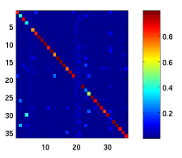
\includegraphics[width=0.2\linewidth]{sensitivity}
\end{figure}

"Simonyan et al. [24], however, demonstrated that DeConvNets can be interpreted as a sensitivity analysis of the network input/output relation." \cite{Mahendran2015}

"the methods proposed in [27], [28] do not explain the decision of a classifier but rather perform sensitivity analysis by computing the gradient of the decision function. This results in an analysis of variations of that function, without however seeking to provide a full explanation why a certain data point has been predicted in a certain way. Specifically, the gradient of a function does not contain information on the saliency of a feature in the data to which the function is applied. Simonyan et al. [24] incorporate saliency information by multiplying the gradient by the actual data point." \cite{Montavon2017}

"Zeiler and Fergus [36], who backtrack the network computations to identify which image patches are responsible for certain neural activations" \cite{Mahendran2015}

"These approaches make perturbations to individual inputs or neurons and observe the impact on later neurons in the network. Zeiler \& Fergus (Zeiler \& Fergus, 2013) occluded different segments of an input image and visualized the change in the activations of later layers. “In-silico muta- genesis” (Zhou \& Troyanskaya, 2015) introduced virtual mutations at individual positions in a genomic sequence and quantified the their impact on the output. Zintgraf et al. (Zintgraf et al., 2017) proposed a clever strategy for analyzing the difference in a prediction after marginalizing over each input patch. However, such methods can be com- putationally inefficient as each perturbation requires a sep- arate forward propagation through the network. They may also underestimate the importance of features that have sat- urated their contribution to the output." \cite{Shrikumar2017}
\begin{figure}[h]
	\centering
	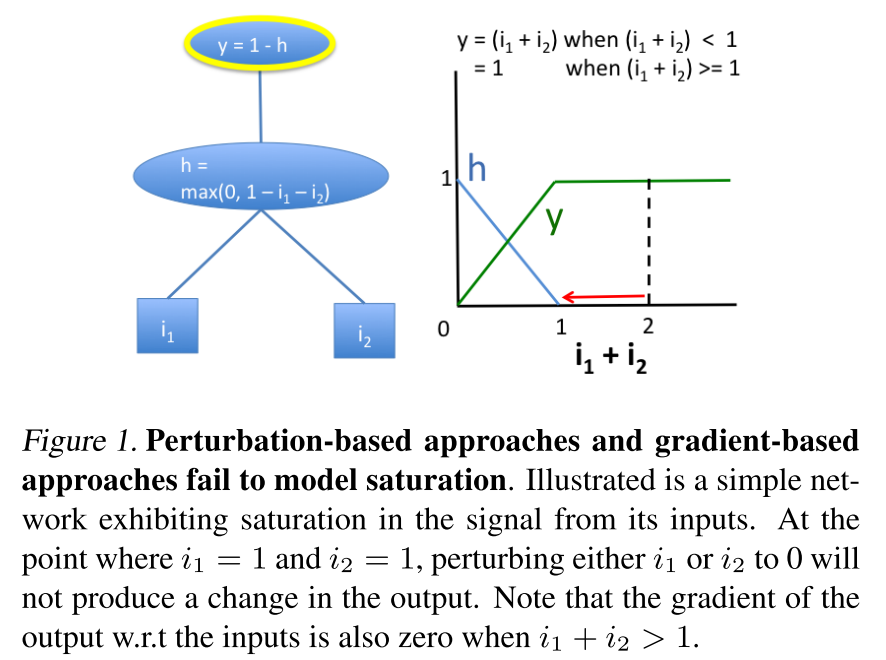
\includegraphics[width=0.6\linewidth]{saturation}
\end{figure}
\subsubsection{Signal masking approach}
"This method was developed along the course of the project in order to evaluate the effect of removing the signal from certain regions of the input sequences. It is a way of assessing, for a trained model, which parts of the input sequence have a higher importance to determine the final classification." \cite{Fontal2017}

\subsection{Backpropagation-based approaches}
"In contrast to perturbation methods, backpropagation approaches are computationally efficient as they propagate an importance signal from the output neuron backwards through the layers towards the input in a single pass.
DeepLIFT belongs to this family of approaches.
[,,,]
\subsubsection{GRADIENTS, DECONVOLUTIONAL NETWORKS AND GUIDED BACKPROPAGATION}
Simonyan et al. \cite{Simonyan2014} proposed using the gradient of the output w.r.t. pixels of an input image to compute a “saliency map” of the image in the context of image classification tasks. The authors showed that this was similar to deconvolutional networks \cite{Zeiler2014} except for the handling of the nonlinearity at rectified linear units (ReLUs). When backpropagating importance using gradients, the gradient coming into a ReLU during the backward pass is zero’d out if the input to the ReLU during the forward pass is negative. By contrast, when backpropagating an importance signal in deconvolutional networks, the importance signal coming into a ReLU during the backward pass is zero’d out if and only if it is neg-ative, with no regard to sign of the input to the ReLU during the forward pass.
Springenberg et al., (Springenberg et al., 2014) combined these two approaches into Guided Backpropagation, which zero’s out the importance signal at a ReLU if either the input to the ReLU during the for-ward pass is negative or the importance signal during the backward pass is negative. Guided Backpropagation can be thought of as equivalent to computing gradients, with the caveat that any gradients that become negative during the backward pass are discarded at ReLUs. Due to the zeroing out of negative gradients, both guided backpropagation and deconvolutional networks can fail to highlight inputs that contribute negatively to the output. Additionally, none of the three approaches would address the saturation problem illustrated in Fig. 1, as the gradient of y w.r.t. h is negative (causing Guided Backprop and deconvolutional networks to assign zero importance), and the gradient of h w.r.t both i1 and i2 is zero when i1 + i2 > 1 (causing both gradients and Guided Backprop to be zero). Discontinuities in the gradients can also cause undesirable artifacts." \cite{Shrikumar2017}
\begin{figure}[h]
	\centering
	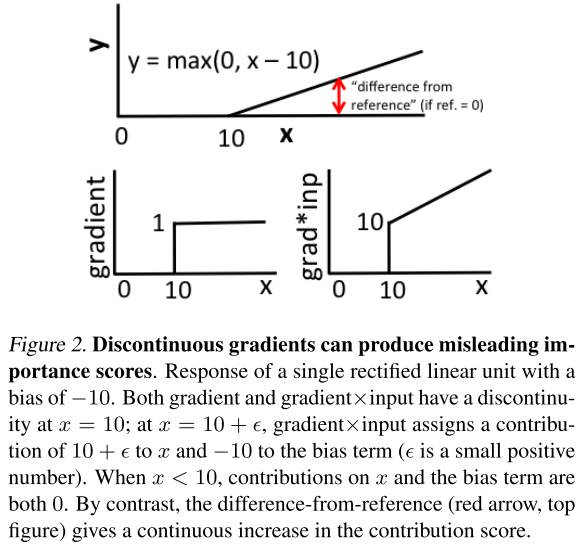
\includegraphics[width=0.6\linewidth]{discontinuity}
\end{figure}
\subsubsection{LAYERWISE RELEVANCE PROPAGATION AND GRADIENT × INPUT}
"Bach et al. (Bach et al., 2015) proposed an approach for propagating importance scores called Layerwise Relevance Propagation (LRP).

Shrikumar et al. and Kindermans et al. (Shrikumar et al., 2016; Kindermans et al., 2016) showed that absent modifications to deal with numerical stability, the original LRP rules were equivalent within a scaling factor to an elementwise product between the saliency maps of Simonyan et al. and the input (in other words, gradient × input).
[...]
While gradient × input is often preferable to gradients alone as it leverages the sign and strength of the input, it still does not address the saturation problem in Fig. 1 or the thresholding artifact in Fig. 2." \cite{Shrikumar2017}
\subsubsection{INTEGRATED GRADIENTS}
"Instead of computing the gradients at only the current value of the input, one can integrate the gradients as the inputs are scaled up from some starting value (eg: all zeros) to their current value (Sundararajan et al., 2016). This ad- dressess the saturation and thresholding problems of Fig. 1 and Fig. 2, but numerically obtaining high-quality inte- grals adds computational overhead. Further, this approach can still give highly misleading results (see Section 3.4.3)." \cite{Shrikumar2017}

\subsection{DeepLIFT}
"Our approach is unique in two regards: first, it frames the question of importance in terms of differences from a ‘reference’ state, where the ‘reference’ is chosen by the user according to what is appropriate for the problem at hand. In contrast to most gradient-based methods, using a difference-from-reference allows DeepLIFT to propagate an importance signal even in situations where the gradient is zero and avoids artifacts caused by discontinuities in the gradient. Second, by optionally giving separate consideration to the effects of positive and negative contributions at nonlinearities, DeepLIFT can reveal dependencies missed by other approaches. As DeepLIFT scores are com- puted using a backpropagation-like algorithm, they can be obtained efficiently in a single backward pass through the network after a prediction has been made." \cite{Shrikumar2017}

\subsection{Deep Taylor Decomposition}
"The main goal of this paper is to reconcile the functional and rule-based approaches for obtaining these decompositions, in a similar way to the error backpropagation algorithm [23] that also has a functional and a message passing interpretation. We call the resulting framework deep Taylor decomposition. This new technique seeks to replace the analytically intractable standard Taylor decomposition problem by a multitude of simpler analytically tractable Taylor decompositions—one per neuron.
[...]
Our method is based on deep Taylor decomposition and efficiently utilizes the structure of the network by backpropagating the explanations from the output to the input layer.
[...]
In this paper, we focus instead on the interpretation of the prediction of individual data points, for which portions of the trained model may either be relevant or not relevant.
[...]
The classification decision is first decomposed in terms of contributions R1, R2, R3 of respective hidden neurons x1, x2, x3, and then, the contribution of each hidden neuron is independently redistributed onto the pixels, leading to a relevance map (or heatmap) in the pixel space, that explains the classification “0”.
A main result of this work is the observation that application
of deep Taylor decomposition to neural networks used for image classification, yields rules that are similar to those proposed by [22] (the αβ-rule and the ?-rule), but with specific instantiations of their hyperparameters, previously set heuristically." \cite{Montavon2017}

\subsection{In biological sequences}
"Our first visualization method is finding a test sequence’s saliency map which uses first-order derivatives to describe the importance of each nucleotide in making the final prediction. [...] we seek to visualize the influence of each position (i.e. nucleotide) on the prediction. Our approach is similar to the methods used on images by \cite{Simonyan2014} and Baehrens et al.[4]. Given a sequence X0 of length |X0|, and class c ∈ C, a DNN model provides a score function Sc(X0). We rank the nucleotides of X0 based on their influence on the score Sc(X0). Since Sc(X) is a highly non-linear function of X with deep neural nets, it is hard to directly see the influence of each nucleotide of X on Sc. Mathematically, around the point X0, Sc(X) can be approximated by a linear function by computing the first-order Taylor expansion:
Sc(X) ≈ wTX + b = ?|X| wixi + b
where w is the derivative of Sc with respect to the sequence variable X at the point X0:
w =∂Sc∂X|X0 = saliency map
This derivative is simply one step of backpropagation in the DNN model, and is therefore easy to compute. We do a pointwise multiplication of the saliency map with the one-hot encoded sequence to get the derivative values for the actual nucleotide characters of the sequence (A,T,C, or G) so we can see the influence of the character at each position on the output score. Finally, we take the element-wise magnitude of the resulting derivative vector to visualize how important each character is regardless of derivative direction. We call the resulting vector a “saliency map[21]” because it tells us which nucleotides need to be changed the least in order to affect the class score the most. As we can see from equation 5, the saliency map is simply a weighted sum of the input nucleotides, where the each weight, wi, indicates the influence of that nucleotide position on the output score.
[...]
From each positive test sequence (thus, 500 total for each TF dataset) we extract a motif from the saliency map by selecting the contiguous length-9 subsequence that achieves the highest sum of contiguous length-9 saliency map values." \cite{Lanchantin2016}


\section{Model inversion}

"A common hypothesis is that representations collapse irrelevant differences in images (e.g. illumination or viewpoint), so that Φ should not be uniquely invertible.
Hence, we pose this as a reconstruction problem and find a number of possible reconstructions rather than a single one. By doing so, we obtain insights into the invariances captured by the representation." \cite{Mahendran2015}

"This is formulated as the problem of finding an image whose representation best matches the one given [34]. Formally, given a representation function Φ : RH×W×C → Rd and a representation Φ0 = Φ(x0) to be inverted, reconstruction finds the image x ∈ RH×W×C that minimizes the objective: x∗ = argmin ?(Φ(x), Φ0) + λR(x) (1) x∈RH×W×C
where the loss ? compares the image representation Φ(x) to the target one Φ0 and R : RH×W×C → R is a regulariser capturing a natural image prior. Minimising (1) results in an image x∗ that “resembles”
x0 from the viewpoint of the representation. While there may be no unique solution to this problem, sampling the space of possible reconstructions can be used to characterise the space of images that the representation deems to be equivalent, revealing its invariances." \cite{Mahendran2015}

\section{Hard-negative mining}

"We make the connection with hard-negative mining explicitly, as it is close in spirit: hard-negative mining, in computer vision, consists of identifying training set examples (or portions thereof) which are given low probabilities by the model, but which should be high probability instead, cf. [5]. The training set distribution is then changed to emphasize such hard negatives and a further round of model training is performed. As shall be described, the optimization problem proposed in this work can also be used in a constructive way, similar to the hard-negative mining principle." \cite{Szegedy2013}

\section{Sample methods}
\subsection{\cite{Olah2017}}
"Images were optimized for 2560 steps in a color-decorrelated fourier-transformed space, using Adam at a learning rate of 0.05. We used each of following transformations in the given order at each step of the optimization:

Padding the input by 16 pixels to avoid edge artifacts

Jittering by up to 16 pixels

Scaling by a factor randomly selected from this list: 1, 0.975, 1.025, 0.95, 1.05

Rotating by an angle randomly selected from this list; in degrees: -5, -4, -3, -2, -1, 0, 1, 2, 3, 4, 5

Jittering a second time by up to 8 pixels

Cropping the padding" \cite{Olah2017}

\bibliography{bib}{}
\bibliographystyle{apalike}


\end{document}
